\documentclass[a4paper,ngerman,landscape,12pt]{scrartcl}

\usepackage[utf8]{inputenc}

\usepackage[ngerman]{babel}
\usepackage{hyperref}

\usepackage{graphicx,ragged2e}

\usepackage[protrusion=true,expansion=true]{microtype}

\usepackage{libertine}
\usepackage{tabto}

\setlength\parskip{\medskipamount}
\setlength\parindent{0pt}

\usepackage{geometry}
\geometry{tmargin=0.7cm,bmargin=0.3cm,lmargin=2.5cm,rmargin=2.5cm}

\pagestyle{empty}

\begin{document}

\begin{center}
  \Huge
  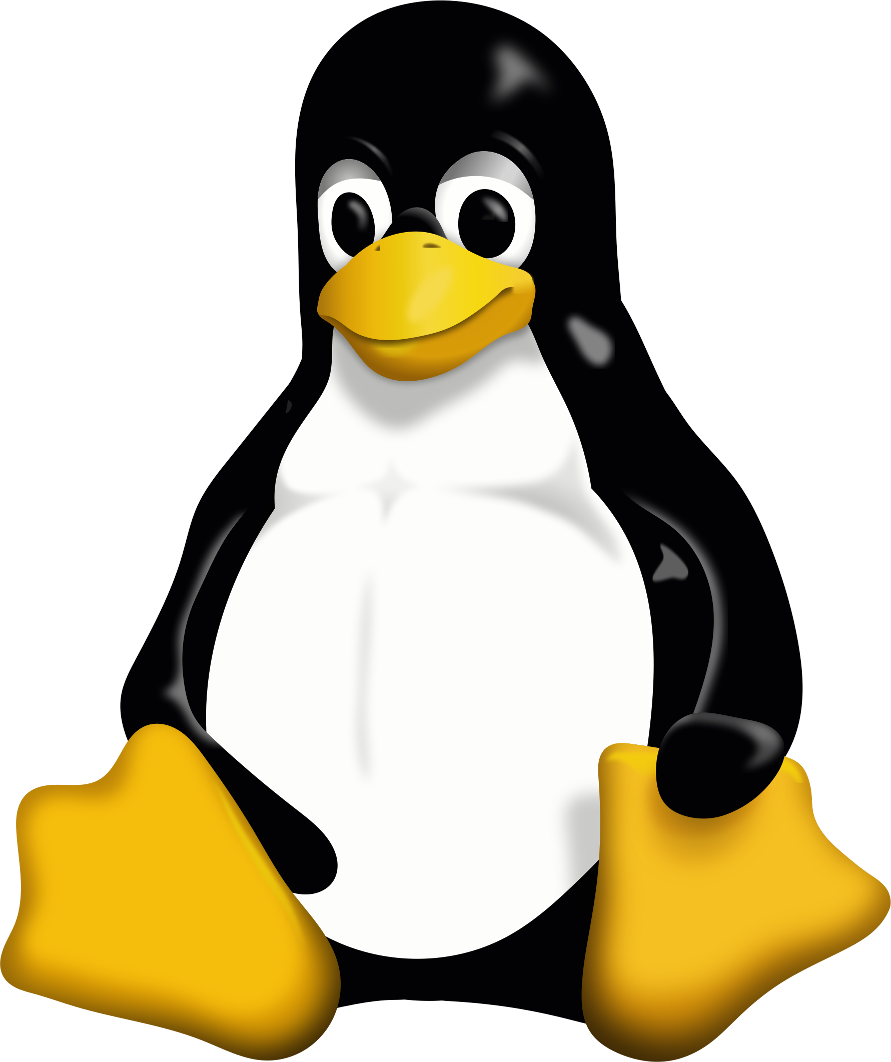
\includegraphics[height=0.2\textheight]{tux}\quad
  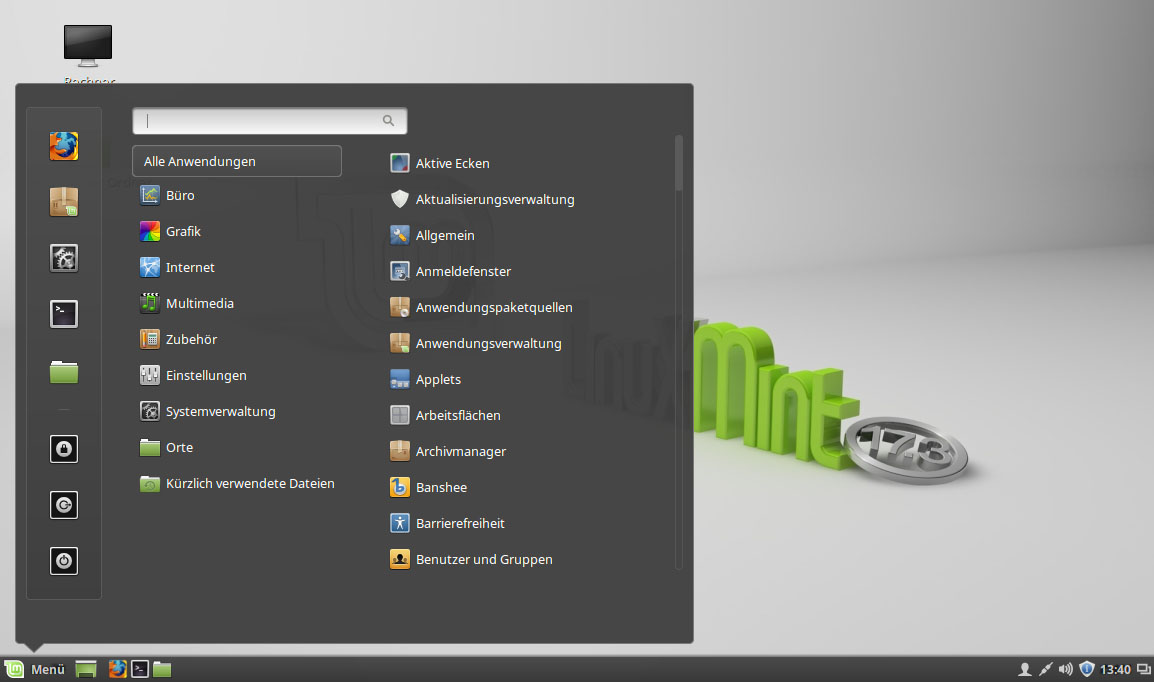
\includegraphics[height=0.2\textheight]{linux-mint}\quad
  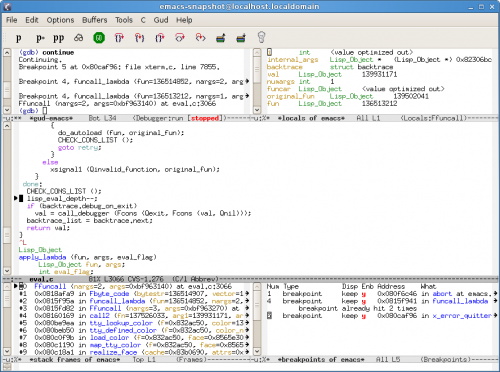
\includegraphics[height=0.2\textheight]{linux-developing}\quad
  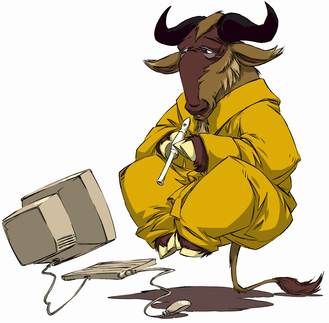
\includegraphics[height=0.2\textheight]{gnu}

  Freitag, 20. Oktober 2017, 15:15 Uhr, 2004/L1 \\
  \mbox{\textbf{Linux-Installationsparty}}

  \Large
  \begin{minipage}{0.99\textwidth}
    \setlength\parskip{\medskipamount}
    \vspace{0.3em}
    \begin{itemize}
      \item Freie Alternative zu Microsoft Windows und Apple Mac OS X.
      Entwickelt von ehrenamtlichen Freiwilligen auf der ganzen Welt,
      auch einigen Studierenden der Uni Augsburg. Kostet nichts.
      \item Läuft insbesondere auf älteren Rechnern flott, deutlich schneller
      als Windows.
      \item Tronjaner für Linux sind eine akademische Kuriosität. Man
      kann ganz unbedarft surfen.
      \item Mit Linux kann man leichter in die Programmierung einsteigen.
      Quelltexte für Linux und alle Linux-Programme sind online verfügbar: zum
      Selbststudium und um etwaige eigene Verbesserungen mit der Welt zu
      teilen.
      \item Linux nervt nicht: Es gibt es keine stundenlangen "`Schalten Sie
      den Computer nicht aus"'-Updates. Sicherheitsupdates werden über eine
      nicht-nervige Art und Weise eingespielt.
      \item Linux bringt auf der Straße mehr Ansehen (street credibility).
      Fast alle Lehrstühle im Mathegebäude verwenden Linux.
    \end{itemize}
  \end{minipage}
  \justifying

  \noindent
  \normalsize
  Interessiert? Bei der Linux-Installationsparty siehst du, wie Linux in Aktion
  aussieht, und kannst es, wenn du möchtest, gleich auf deinem eigenen Rechner
  installieren. Beim Starten kann man dann zwischen Linux und Windows
  auswählen. Die Bedienung von Linux ist kinderleicht. Zur Installation ist
  dagegen die Erfahrung, die wir mitbringen, nicht ganz unnütz, weil es nicht
  so leicht ist, den Rechner zu überreden, den Installationsstick zu verwenden.
  Schau bei Interesse einfach vorbei. :-)

  \noindent
  Organisiert für: alle, die Linux ansehen oder installieren wollen,
  insbesondere euch neue Erstsemesterstudierende. Willkommen an der Uni
  Augsburg!
  Organisiert von: Ingo und vielen anderen Studierenden
\end{center}

\end{document}
